%% -*- coding:utf-8 -*-
\chapter{Clang architecture}
\pagestyle{fancy}
\fancyhf{}
\rhead{\thepage}
\lhead{Clang architecture}

In this chapter, we will examine the internal architecture of Clang and its
relationship with other LLVM components. We will begin with an overview of the
overall compiler architecture, with a specific focus on the clang driver. As the
backbone of the compiler, the driver runs all compilation phases and controls
their execution. Finally, we will concentrate on the frontend portion of the
Clang compiler, which includes lexical and semantic analysis, and produces an
Abstract Syntax Tree (\myast) as its primary output. The \myast forms the
foundation for most clang tools, and we will examine it more closely in the next
chapters. 

The following topics will be covered in this chapter:
\begin{itemize}
\item Compiler overview
\item Clang driver overview, including an explanation of the compilation phases
  and their execution 
\item Clang frontend overview, which covers frontend actions, preprocessor,
  parser, and sema 
\end{itemize}

\section{Compilers overview}
\label{sec:compiler_overview}
Despite the fact that compilers are used to translate programs from one form to
another, they can also be considered as large software systems that use various
algorithms and data structures. The knowledge obtained from studying compilers
is not specific to compilers and can be applied to other software as well. On
the other hand, compilers are also a subject of active scientific research, and
there are many unexplored areas and topics to investigate. 

You can find some basic information about the internal structure of a compiler
here. We will keep it as basic as possible so the information is applicable
to any compiler, not just Clang. We will briefly cover all phases of
compilation, which will help to understand Clang's position in the overall
compiler architecture.

\subsection{Compiler workflow}

The primary function of a compiler is to convert a program written in a specific
programming language (such as C/C++ or FORTRAN) into a format that can be
executed on a target platform. This process involves the use of a compiler,
which takes the source file and any compilation flags, and produces a build
artifact, such as an executable or object file, as shown in
\cref{fig:compiler}. 
\begin{figure}
  \begin{center}
    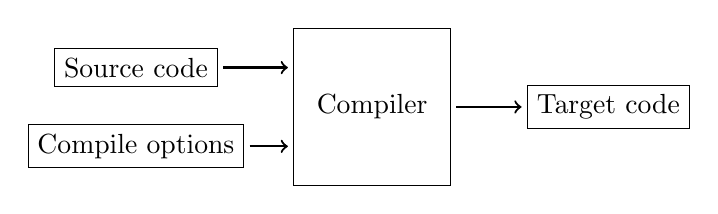
\begin{tikzpicture}
      \node[rectangle,draw] (source) at (-1,1.5) {Source code};
      \draw[->,thick,shorten <=2pt,shorten >=2pt] (source) to (1,1.5);
      \node[rectangle,draw] (flags) at (-1,0.5) {Compile options};
      \draw[->,thick,shorten <=2pt,shorten >=2pt] (flags) to (1,0.5);
      \node[rectangle] (compiler) at (2,1) {Compiler};
      \draw (1,0) -- (3,0) -- (3,2) -- (1,2) -- (1,0);
      \node[rectangle,draw] (target) at (5,1) {Target code};
      \draw[->,thick,shorten <=2pt,shorten >=2pt] (3,1) to (target);
    \end{tikzpicture}
  \end{center}
  \caption{Compiler takes source code and compile options and transform them
    into a code on the target platform}
  \label{fig:compiler}
\end{figure}
The term "target platform" can have a broad meaning. It can refer to machine
code that is executed on the same host, as is typically the case. But it can
also refer to cross-compilation, where the compiler generates code for a
different computer architecture than the host. For example, code for a mobile
application or embedded application running on ARM can be generated using an
Intel machine as the host. Additionally, the target platform is not limited to
machine code only. For example, some early C++ compilers (such as "cc") would
produce pure C code as output. This was done because, at the time, C was the
most widely used and well-established programming language, and the C compiler
was the most reliable way to generate machine code. This approach allowed early
C++ programs to be run on a wide range of platforms since most systems already
had a C compiler available. The produced C code could then be compiled into
binary by another compiler.   

\begin{figure}
  \begin{center}
    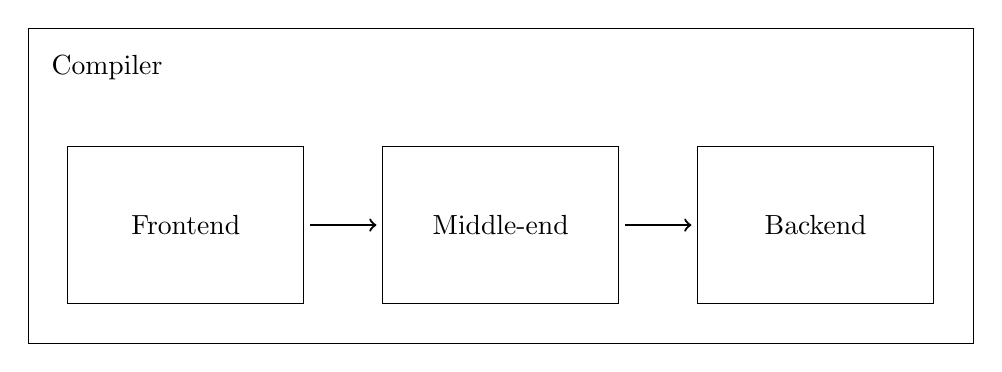
\begin{tikzpicture}
      \node[rectangle] (compiler) at (1,3.5) {Compiler};
      \draw (0,0) -- (12,0) -- (12,4) -- (0,4) -- (0,0);
      \node[rectangle,draw,minimum height = 2cm, minimum width = 3cm] (frontend)
      at (2,1.5) {Frontend}; 
      \node[rectangle,draw,minimum height = 2cm, minimum width = 3cm]
      (middleend) at (6,1.5) {Middle-end}; 
      \node[rectangle,draw,minimum height = 2cm, minimum width = 3cm] (backend)
      at (10,1.5) {Backend};
      \draw[->,thick,shorten <=2pt,shorten >=2pt] (frontend) to (middleend);
      \draw[->,thick,shorten <=2pt,shorten >=2pt] (middleend) to (backend);
    \end{tikzpicture}
  \end{center}
  \caption{Typical compiler workflow: source program is passed via different
    stages: frontend, middle-end and backend}
  \label{fig:compiler_workflow}
\end{figure}

We are going to focus on compilers that produce binary code, and a typical
compiler workflow for such a compiler is shown in
\cref{fig:compiler_workflow}. The stages of compilation can be described as
follows: 
\begin{itemize}
\item Frontend: The Frontend does lexical analysis and parsing, which includes
  both syntax analysis and semantic analysis. The syntax analysis assumes that
  your program is well-organized according to the language grammar rules. The
  semantic analysis performs checks on the program's meaning and rejects invalid
  programs, such as those that use wrong types. 
\item Middle-end: The Middle-end performs various optimizations on the
  intermediate representation (IR) code (LLVM-IR for clang). 
\item Backend: The Backend of a compiler takes the optimized or transformed
  IR and generates machine code or assembly code that can be executed by the
  target platform. 
\end{itemize} 

The source program is transformed into different forms as it passes through the
various stages. For example, the Frontend produces IR code, which is then
optimized by the Middle-end and finally converted into native code by the
Backend (see \cref{fig:source_code_transformation}). 
\begin{figure}
  \begin{center}
    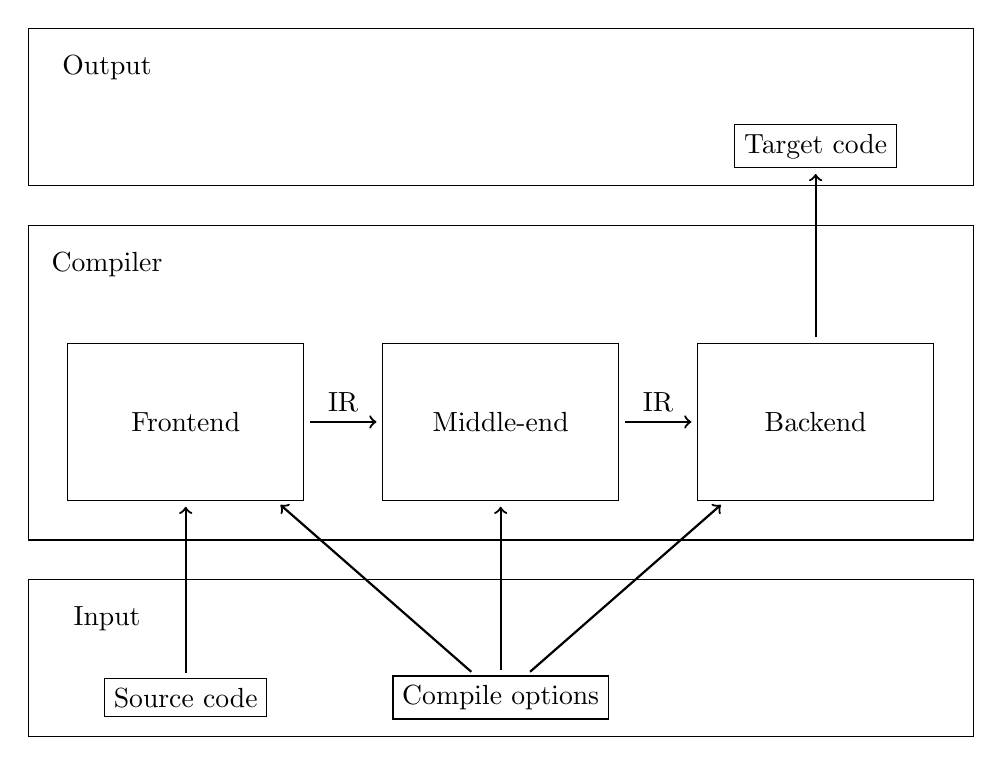
\begin{tikzpicture}
      \node[rectangle] (compiler) at (1,3.5) {Compiler};
      \draw (0,0) -- (12,0) -- (12,4) -- (0,4) -- (0,0);
      \node[rectangle,draw,minimum height = 2cm, minimum width = 3cm] (frontend)
      at (2,1.5) {Frontend}; 
      \node[rectangle,draw,minimum height = 2cm, minimum width = 3cm]
      (middleend) at (6,1.5) {Middle-end}; 
      \node[rectangle,draw,minimum height = 2cm, minimum width = 3cm] (backend)
      at (10,1.5) {Backend};
      \draw[->,thick,shorten <=2pt,shorten >=2pt] (frontend) to
      node[pos=0.5,above]{IR} (middleend); 
      \draw[->,thick,shorten <=2pt,shorten >=2pt] (middleend) to
      node[pos=0.5,above]{IR} (backend);
      \node[rectangle] (input) at (1,-1) {Input};
      \draw (0,-2.5) -- (12,-2.5) -- (12,-0.5) -- (0,-0.5) -- (0,-2.5);      
      \node[rectangle,draw] (source) at (2,-2) {Source code};
      \draw[->,thick,shorten <=2pt,shorten >=2pt] (source) to (frontend);
      \node[rectangle,draw] (options) at (6,-2) {Compile options};
      \draw[->,thick,shorten <=2pt,shorten >=2pt] (options) to (frontend);
      \draw[->,thick,shorten <=2pt,shorten >=2pt] (options) to (middleend);
      \draw[->,thick,shorten <=2pt,shorten >=2pt] (options) to (backend);
      \node[rectangle] (output) at (1,6) {Output};
      \draw (0,4.5) -- (12,4.5) -- (12,6.5) -- (0,6.5) -- (0,4.5);
      \node[rectangle,draw] (target) at (10,5) {Target code};
      \draw[->,thick,shorten <=2pt,shorten >=2pt] (backend) to (target);
    \end{tikzpicture}
  \end{center}
  \caption{Source code transformation by compiler: Input data consists of
    \textit{Source code} and \textit{Compile options}. The source code is
    transformed by \textit{Frontend} into IR (Intermediate representation).
    \textit{Middle-end} does different optimizations on IR and passes the final
    (optimazed) result to \textit{Backend}. \textit{Backend} generates the
    \textit{Target code}.
    Frontend, Middle-end and Backend use \textit{Compile options} as setting for
    the code transformations}  
  \label{fig:source_code_transformation}
\end{figure}

\subsection{Frontend}

Our primary focus will be on the frontend, so we will examine its
components. The frontend also transforms the source code into various forms
before it produces the IR. The first component of the frontend is the \lexer
(see \cref{fig:compiler_frontend}). It converts the source code into a set of
tokens, which are used to create a special data structure called the abstract
syntax tree (\myast). The final component, code generator (Codegen), traverses
the \myast and generates the IR from it. 

\begin{figure}
  \begin{center}
    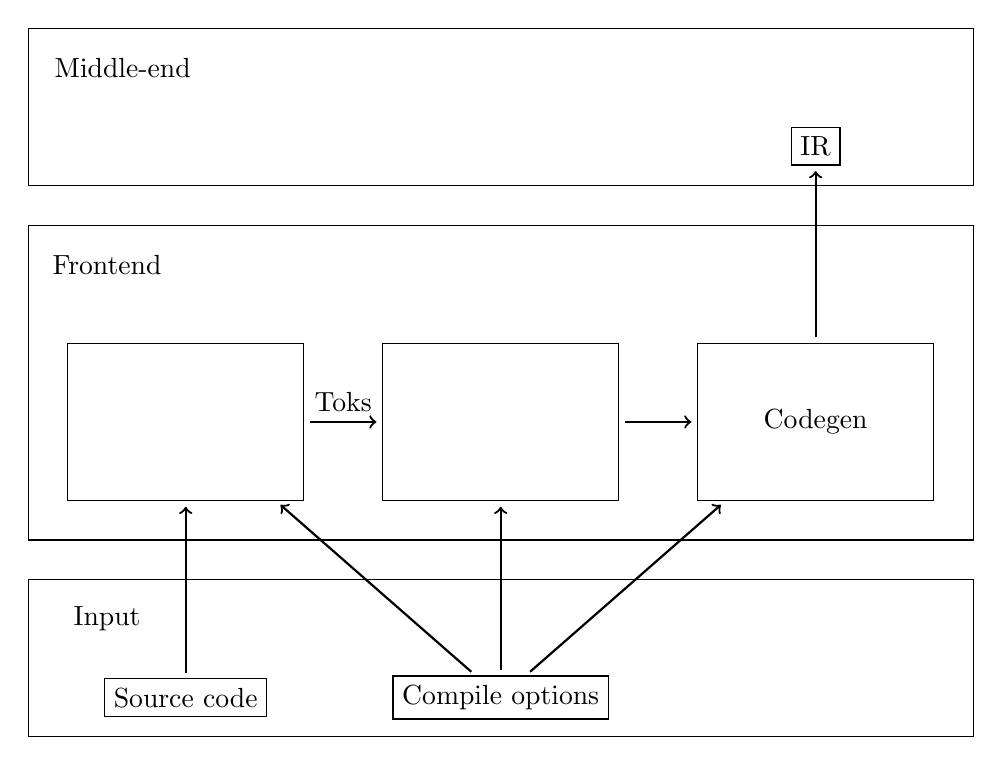
\begin{tikzpicture}
      \node[rectangle] (frontend) at (1,3.5) {Frontend};
      \draw (0,0) -- (12,0) -- (12,4) -- (0,4) -- (0,0);
      \node[rectangle,draw,minimum height = 2cm, minimum width = 3cm] (lexer)
      at (2,1.5) {\lexer}; 
      \node[rectangle,draw,minimum height = 2cm, minimum width = 3cm]
      (parser) at (6,1.5) {\parser}; 
      \node[rectangle,draw,minimum height = 2cm, minimum width = 3cm] (codegen)
      at (10,1.5) {Codegen};
      \draw[->,thick,shorten <=2pt,shorten >=2pt] (lexer) to
      node[pos=0.5,above]{Toks} (parser); 
      \draw[->,thick,shorten <=2pt,shorten >=2pt] (parser) to
      node[pos=0.5,above]{\myast} (codegen);
      \node[rectangle] (input) at (1,-1) {Input};
      \draw (0,-2.5) -- (12,-2.5) -- (12,-0.5) -- (0,-0.5) -- (0,-2.5);      
      \node[rectangle,draw] (source) at (2,-2) {Source code};
      \draw[->,thick,shorten <=2pt,shorten >=2pt] (source) to (lexer);
      \node[rectangle,draw] (options) at (6,-2) {Compile options};
      \draw[->,thick,shorten <=2pt,shorten >=2pt] (options) to (lexer);
      \draw[->,thick,shorten <=2pt,shorten >=2pt] (options) to (parser);
      \draw[->,thick,shorten <=2pt,shorten >=2pt] (options) to (codegen);
      \node[rectangle] (output) at (1.2,6) {Middle-end};
      \draw (0,4.5) -- (12,4.5) -- (12,6.5) -- (0,6.5) -- (0,4.5);
      \node[rectangle,draw] (target) at (10,5) {IR};
      \draw[->,thick,shorten <=2pt,shorten >=2pt] (codegen) to (target);
    \end{tikzpicture}
  \end{center}
  \caption{Compiler frontend: source code is transformed into a set of tokens
    (Toks) by \lexer. \parser takes the tokens and creates Abstract syntax tree
    (\myast). Codegen generates IR from \myast} 
  \label{fig:compiler_frontend}
\end{figure}

We will use a simple C/C++ program that calculates the maximum of two numbers to
demonstrate the workings of the Frontend. The code for the program is as
follows: 
\begin{figure}[H]
\inputminted{c++}{./src/part1/ch2_arch/max.cpp}
\caption{Test program for compiler frontend investigations}
\label{fig:arch_max}
\end{figure}
\subsubsection{Lexer}

The Frontend process starts with the \lexer, which converts the input source
into a stream of tokens. In our example program (see \cref{fig:arch_max}), the
first token is the keyword \myshell{int}, which represents the integer
type. This is followed by the identifier \myshell{max} for the function
name. The next token is the left parenthesis \myshell{(}, and so on (see
\cref{fig:lexer}). 
\begin{figure}
  \begin{center}
    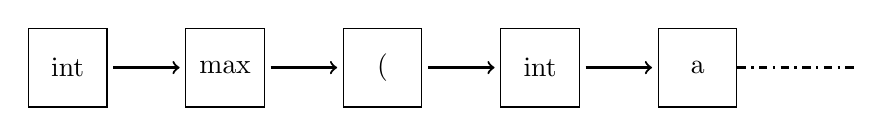
\begin{tikzpicture}
      \node[rectangle,draw,minimum height = 1cm, minimum width = 1cm] (int1) at
      (0,0) {int}; 
      \node[rectangle,draw,minimum height = 1cm, minimum width = 1cm] (max) at
      (2,0) {max}; 
      \node[rectangle,draw,minimum height = 1cm, minimum width = 1cm] (lpar) at
      (4,0) {(}; 
      \node[rectangle,draw,minimum height = 1cm, minimum width = 1cm] (int2) at
      (6,0) {int}; 
      \node[rectangle,draw,minimum height = 1cm, minimum width = 1cm] (a) at
      (8,0) {a}; 
      \draw[->,thick,shorten <=2pt,shorten >=2pt] (int1) to (max);
      \draw[->,thick,shorten <=2pt,shorten >=2pt] (max) to (lpar);
      \draw[->,thick,shorten <=2pt,shorten >=2pt] (lpar) to (int2);
      \draw[->,thick,shorten <=2pt,shorten >=2pt] (int2) to (a);
      \draw[thick,dash dot] (a) to (10,0);
    \end{tikzpicture}
  \end{center}
  \caption{\lexer: the program source is converted into a stream of tokens} 
  \label{fig:lexer}
\end{figure}

\subsubsection{Parser}
The \parser is the next component following the \lexer. The primary output
produced by the \parser is called as abstract syntax tree (AST). This tree
represents the abstract syntactic structure of the source code written in a
programming language. The \parser generates the AST by taking the stream of
tokens produced by the \lexer as input and organizing them into a tree-like
structure. Each node in the tree represents a construct in the source code, such
as a statement or expression, and the edges between nodes represent the
relationships between these constructs. 

\begin{center}
  \begin{figure}
    \resizebox{.9\linewidth}{!}{\
      \begin{forest}
        for tree={draw, rounded corners=5mm, font=\sffamily,
          minimum width=2cm, minimum height=1cm,
          forked edge, edge={blue,-latex},
          s sep=2cm, l sep=1cm, fork sep=5mm}
        [Function: max [Parameter: a][Parameter: b][Statement:
            \myshell{compound}[Statement: \myshell{if}[Binary operator:
                >[Variable: \myshell{a}][Variable: \myshell{b}]][Statement:
                \myshell{return}[Variable: \myshell{a}]]][Statement:
              \myshell{return}[Variable: \myshell{b}]]]] 
      \end{forest}
    }
    \caption{The AST for our example program that calculates maximum of 2 numbers
    }  
    \label{fig:ast}
  \end{figure}
\end{center}

The AST for our example program is shown in \cref{fig:ast}. As you can see, our
function (\myshell{max}) has two parameters (\myshell{a} and \myshell{b}) and a
body. The body is marked as a compound statement in \cref{fig:ast}. The compound
statement consists of other statements, such as \myshell{return} and
\myshell{if}. The variables \myshell{a} and \myshell{b} are used in the bodies
of these statements. You may also be interested in the real AST generated by
\clang for the compound statement, the result of which is shown in
\cref{fig:ast2}. 

\begin{center}
  \begin{figure}
    \digraph[width=1.0\textwidth] {unnamed} {
      Node0x10277088 [shape=record,label="{CompoundStmt}"];
      Node0x10277088 -> Node0x10277020;
      Node0x10277088 -> Node0x10277078;
      Node0x10277020 [shape=record,label="{IfStmt}"];
      Node0x10277020 -> Node0x10276fb8;
      Node0x10277020 -> Node0x10277010;
      Node0x10276fb8 [shape=record,label="{BinaryOperator}"];
      Node0x10276fb8 -> Node0x10276f88;
      Node0x10276fb8 -> Node0x10276fa0;
      Node0x10276f88 [shape=record,label="{ImplicitCastExpr}"];
      Node0x10276f88 -> Node0x10276f48;
      Node0x10276f48 [shape=record,label="{DeclRefExpr}"];
      Node0x10276fa0 [shape=record,label="{ImplicitCastExpr}"];
      Node0x10276fa0 -> Node0x10276f68;
      Node0x10276f68 [shape=record,label="{DeclRefExpr}"];
      Node0x10277010 [shape=record,label="{ReturnStmt}"];
      Node0x10277010 -> Node0x10276ff8;
      Node0x10276ff8 [shape=record,label="{ImplicitCastExpr}"];
      Node0x10276ff8 -> Node0x10276fd8;
      Node0x10276fd8 [shape=record,label="{DeclRefExpr}"];
      Node0x10277078 [shape=record,label="{ReturnStmt}"];
      Node0x10277078 -> Node0x10277060;
      Node0x10277060 [shape=record,label="{ImplicitCastExpr}"];
      Node0x10277060 -> Node0x10277040;
      Node0x10277040 [shape=record,label="{DeclRefExpr}"];
    }
    \caption{The AST for compound statement generated by \clang. The tree
      generated by \myshell{clang -cc1 -ast-view <...>} command} 
    \label{fig:ast2}
  \end{figure}
\end{center}

The \parser performs two activities:
\begin{enumerate}
\item Syntax analysis: the \parser constructs the \myast by analyzing the syntax
  of the program. 
\item Semantic analysis: the \parser analyzes the program semantically.
\end{enumerate}

One of the primary goals of analysis is error detection, and the \parser
produces an error message if it fails in syntax or semantic analysis. We can get
a sense of this by considering what types of errors are detected by syntax
analysis and which ones are detected by semantic analysis. 

Syntax analysis assumes that the program should be correct in terms of the
grammar specified for the language. For example, the following program is
invalid in terms of syntax because a semicolon is missing at the last return
statement: 

\inputminted{c++}{./src/part1/ch2_arch/max_invalid_syntax.cpp}

\clang produces the following output for the program:
\begin{adjustwidth}{0em}{0em}
\begin{verbatim}
max_invalid_syntax.cpp:4:11: error: expected ';' after return statement
  return b // missing ;
          ^
          ;
\end{verbatim}
\end{adjustwidth}

On the other hand, a program can be syntactically correct but have no sense. The
\parser should detect a semantic error in such cases. For instance, the
following program has a semantic error related to the wrongly used type for the
return value: 
\inputminted{c++}{./src/part1/ch2_arch/max_invalid_sema.cpp}
\clang produces the following output for the program:
\begin{adjustwidth}{0em}{0em}
\begin{verbatim}
max_invalid_sema.cpp:4:10: error: cannot initialize return object of type \
'int' with an rvalue of type 'int *'
  return &b; // invalid return type
         ^~
\end{verbatim}
\end{adjustwidth}

AST is mainly constructed as a result of syntax analysis, but for certain
languages, such as C++, semantic analysis is also crucial for constructing the
AST, particularly for C++ template instantiation. 

During syntax analysis, the compiler verifies that the template declaration
adheres to the language's grammar and syntax rules, including the proper use of
keywords such as "template" and "typename", as well as the formation of the
template parameters and body. 

Semantic analysis, on the other hand, involves the compiler performing template
instantiation, which generates the AST for specific instances of the
template. It's worth noting that the semantic analysis of templates can be quite
complex, as the compiler must perform tasks such as type checking, name
resolution, and more for each template instantiation. Additionally, the
instantiation process can be recursive and lead to a significant amount of code
duplication, known as code bloat. To combat this, C++ compilers employ
techniques such as template instantiation caching to minimize the amount of
redundant code generated. 

\subsubsection{Codegen}
The Codegen
\footnote{
It's worth mentioning that we also have another Codegen component as a part of
Backend that generate the target code.
}
or code generator,
which is the final component of the compiler's frontend, has the primary goal of
generating the Intermediate Representation (IR). For this purpose, the compiler
traverses the AST generated by the parser and converts it into another source
code that is called the Intermediate Representation or IR. The IR is a
language-independent representation, allowing the same middle-end component to
be used for different frontends (FORTRAN vs C++). 

The use of Intermediate Representations (IRs) in compilers is a concept that has
been around for several decades. The idea of using an intermediate
representation to represent the source code of a program during compilation has
evolved over time, and the exact date when IR was first introduced in compilers
is not clear. 

However, it is known that the first compilers in the 1950s and 1960s did not use
IRs and instead translated source code directly into machine code. By the 1960s
and 1970s, researchers had begun experimenting with using IRs in compilers to
improve the efficiency and flexibility of the compilation process. 

One of the first widely used IRs was the three-address code, which was used in
the mid-1960s in IBM/360's FORTRAN compiler. Other early examples of IRs include
the register transfer language (RTL) and the static single assignment (SSA)
form, which were introduced in the 1970s and 1980s respectively. 

Today, the use of IRs in compilers is a standard practice, and many compilers
use multiple IRs throughout the compilation process. This allows for more
powerful optimization and code generation techniques to be applied. 


\section{Clang driver overview}
\label{sec:clang_driver}
When discussing compilers, we typically refer to a command-line utility that
initiates and manages the compilation process. For example, to use the GNU
Compiler Collection, one must call \myshell{gcc} to start the compilation
process. Similarly, to compile a C++ program using Clang, one must call
\myshell{clang} 
as the compiler. The program that controls the compilation process is known as
the driver. The driver coordinates different stages of compilation and connects
them together. In the book, we will be focusing on LLVM and using clang as
the driver for the compilation process. 

It may be confusing for readers that the same word, "clang," is used to refer to
both the compiler front-end and the compilation driver. In contrast, with GCC,
the driver and C++ compiler are separate executables
\footnote{The C/C++ compiler
in GCC is a separate executable called "cc"}.
However, "clang" is a single
executable that functions as both the driver and the compiler front-end. To use
\clang as the compiler front-end only, the special option \myshell{-cc1} must be
passed to it. 

\subsection{Example program}
We will use the simple ``Hello world!'' example program for our experiments with
clang driver. The main source file is called as \myshell{hello.cpp}. The
file implements a trivial C++ program that prints ``Hello world!'' to the standard
output: 
\inputminted{c++}{./src/part1/ch2_arch/hello.cpp}

You can compile the source with
% ./llvm-project-16.x/build/bin/clang src/part1/ch2_arch/hello.cpp -o /tmp/hello -lstdc++
\begin{figure}[H]
\begin{minted}{shell-session}
$ clang hello.cpp -o /tmp/hello -lstdc++
\end{minted}
\caption{Compilation for \myshell{hello.cpp}: We use \myshell{clang} executable as
  the compiler. We also use standard C++ library i.e. we link the
  executable 
  with \myshell{-lstdc++}. The result is stored at \myshell{/tmp/hello}}
\label{fig:hello_compilation}
\end{figure}
As you may see, we specified \myshell{-lstc++} library option because we used
\mintinline{c++}{<iostream>} header from the standard C++ library. We also
specified the output for executable (\myshell{/tmp/hello}) with \myshell{-o}
option. 

\subsection{Compilation phases}
We used 2 inputs for our example program. The first one is our source code, the
second one is a shared library for standard C++ library. The clang driver should
combine the inputs together, pass them via different phases of compilation
process and finally provide the executable file on the target platform.

\clang uses the same process as shown in \cref{fig:compiler_workflow}. You can
ask \clang to show the phases using \myshell{-ccc-print-phases} additional
argument
% clang src/part1/ch2_arch/hello.cpp -o /tmp/hello -lstdc++ -ccc-print-phases
\begin{adjustwidth}{0em}{0em}
\begin{verbatim}
$ clang hello.cpp -o /tmp/hello -lstdc++ -ccc-print-phases
\end{verbatim}
\end{adjustwidth}
The output for the command is the following
\begin{adjustwidth}{0em}{0em}
\begin{verbatim}
              +- 0: input, "hello.cpp", c++
         +- 1: preprocessor, {0}, c++-cpp-output
      +- 2: compiler, {1}, ir
   +- 3: backend, {2}, assembler
+- 4: assembler, {3}, object
|- 5: input, "1%dM", object
6: linker, {4, 5}, image
\end{verbatim}
\end{adjustwidth}

\begin{figure}
  \begin{center}
    \begin{adjustbox}{totalheight=\textheight-10\baselineskip}
      \begin{tikzpicture}
        \node[rectangle] (input) at (1,-1) {Input};
        \draw[dashed] (0,-2.5) -- (12,-2.5) -- (12,-0.5) -- (0,-0.5) -- (0,-2.5);      
        \node[rectangle, draw, dashed, minimum width = 3cm] (source) at (2,-2)
             {hello.cpp}; 
             \node[rectangle, draw, dashed,minimum width = 3cm] (lib) at (10,-2)
                  {libstdc++}; 

                  \node[rectangle,draw,minimum height = 2cm, minimum width = 3cm] (preprocessor)
                  at (2,1.5) {preprocessor};
                  \node[rectangle,draw, dashed, minimum width = 3cm] (cpp-output)
                  at (6,2) {c++-cpp-output};
                  \node[rectangle,draw,minimum height = 2cm, minimum width = 3cm] (compiler)
                  at (2,4) {compiler};
                  \node[rectangle,draw, dashed, minimum width = 3cm] (ir)
                  at (6,4.5) {ir};
                  \node[rectangle,draw,minimum height = 2cm, minimum width = 3cm] (backend)
                  at (2,6.5) {backend};
                  \node[rectangle,draw, dashed, minimum width = 3cm] (asmcode)
                  at (6,7) {assembler};
                  \node[rectangle,draw,minimum height = 2cm, minimum width = 3cm] (assembler)
                  at (2,9) {assembler};
                  \node[rectangle,draw, dashed, minimum width = 3cm] (object)
                  at (6,9.5) {object};

                  \node[rectangle,draw,minimum height = 2cm, minimum width = 3cm] (linker)
                  at (2,11.5) {linker};
                  
                  \node[rectangle] (output) at (1,15.5) {Output};
                  \draw[dashed] (0,14) -- (12,14) -- (12,16) -- (0,16) -- (0,14);      
                  
                  \draw[->,thick,shorten <=2pt,shorten >=2pt] (source) to (preprocessor);
                  \draw[->,thick,shorten <=2pt,shorten >=2pt] (3.5,2) to
                  (cpp-output);
                  \draw[->,thick,shorten <=2pt,shorten >=2pt] (cpp-output) -- (6,3.5) --
                  (3.5,3.5);
                  \draw[->,thick,shorten <=2pt,shorten >=2pt] (3.5,4.5) to (ir);
                  \draw[->,thick,shorten <=2pt,shorten >=2pt] (ir) -- (6,6) --
                  (3.5,6); 
                  \draw[->,thick,shorten <=2pt,shorten >=2pt] (3.5,7) to (asmcode);
                  \draw[->,thick,shorten <=2pt,shorten >=2pt] (asmcode) --
                  (6,8.5) -- (3.5,8.5);
                  \draw[->,thick,shorten <=2pt,shorten >=2pt] (3.5,9.5) to (object);
                  \draw[->,thick,shorten <=2pt,shorten >=2pt] (object) --
                  (6,11) -- (3.5,11); 
                  \draw[->,thick,shorten <=2pt,shorten >=2pt] (lib) --
                  (10,12) -- (3.5,12); 

                  
                  \node[rectangle,draw, dashed, minimum width = 3cm] (image)
                  at (2,14.5) {image};


                  \draw[->,thick,shorten <=2pt,shorten >=2pt] (linker) to (image);
      \end{tikzpicture}
    \end{adjustbox}
  \end{center}
  \caption{Clang driver phases}  
  \label{fig:clang_driver_phases}
\end{figure}

We can visualize the output as shown in \cref{fig:clang_driver_phases}. As we
can see in \cref{fig:clang_driver_phases}, the driver receives an input file
\myshell{hello.cpp}, which is a C++ file. The file is processed by the
preprocessor, and we obtain the preprocessor output (marked as
\myshell{c++-cpp-output}). The result is compiled into IR form by the compiler,
and then the backend converts it into assembly form. This form is later
transformed into an object file. The final object file is combined with another
object (\myshell{libstdc++}) to produce the final binary (\myshell{image}). 


\subsection{Tools execution}
The phases are combined into several tool executions. The Clang driver invokes
different programs to produce the final executable. Specifically, for our
example, it calls the \myshell{clang} compiler and the \myshell{ld} linker. Both
programs require additional arguments that are set up by the driver.  

For instance, our example program (\myshell{hello.cpp}) includes the following
header: 

\begin{minted}{cpp}
#include <iostream>
...
\end{minted}

We have not specified any additional arguments (such as search paths, for
example \myshell{-I}) when we invoked the compilation. However, different
architectures and operating systems might have different paths for locating
headers.  

On Fedora 37, the header is located in the
\myshell{/usr/include/c++/12/iostream} folder. We can examine a detailed
description of the process executed by the driver and the arguments used with
the \mintinline{text}{-###} option: 

% clang src/part1/ch2_arch/hello.cpp -o /tmp/hello -lstdc++ -###
\begin{adjustwidth}{0em}{0em}
\begin{verbatim}
$ clang hello.cpp -o /tmp/hello -lstdc++ -###
\end{verbatim}
\end{adjustwidth}

The output for this command is quite extensive, and certain parts have been
omitted here. Please refer to \cref{fig:driver_tools_execution}. 

\begin{figure}[H]
\begin{minted}{shell-session}
clang version 16.0.0 (https://github.com/llvm/llvm-project.git ...)
 "<...>/llvm-project/build/bin/clang-16"
    "-cc1" ... \
    "-internal-isystem" \
    "/usr/include/c++/12" ... \
    "-internal-isystem" \
    "/usr/include/c++/12/x86_64-redhat-linux" ... \
    "-internal-isystem" ... \
    "<...>/llvm-project/build/lib/clang/16/include" ... \ 
    "-internal-externc-isystem" \
    "/usr/include" ... \
    "-o" "/tmp/hello-XXX.o" "-x" "c++" "hello.cpp"
 ".../bin/ld" ... \
    "-o" "/tmp/hello" ... \
    "/tmp/hello-XXX.o" \
    "-lstdc++" ...
\end{minted}
\caption{Clang driver, tools execution, the host system is Fedora 37.} 
\label{fig:driver_tools_execution}
\end{figure}
As we can see in \cref{fig:driver_tools_execution}, the driver initiates two
processes: \myshell{clang-16} with the \myshell{-cc1} flag (see lines 2-12) and
the linker \myshell{ld} (see lines 13-16). The clang compiler implicitly
receives several search paths, as seen in lines 5, 7, 9 and 11. These paths are
necessary for the inclusion of the iostream header in the test program. The
output of the first executable (\myshell{/tmp/hello-XXX.o}) serves as input for
the second one (see lines 12 and 15). The arguments \myshell{-lstdc++} and
\myshell{-o /tmp/hello} are set for the linker, while the first argument
(hello.cpp) is provided for the compiler invocation (first executable). 

The process can be visualized as shown in
\cref{fig:clang_driver_tools_execution}, where we can see that two executables
are executed as part of the compilation process. The first one is
\myshell{bin/clang-16} with a special flag (\myshell{-cc1}). The second one is
the linker: \myshell{bin/ld}. 

\begin{figure}
  \begin{center}
    \begin{tikzpicture}[node distance = 2cm, auto]
      % Place nodes
      \node [block] (clang) {clang};
      \node [block, below of=clang, right of=clang, node distance=2cm] (clangcc1)
            {clang -cc1};
            \node [block, below of=clangcc1] (ld) {ld};
            % Draw edges
            \path [line] (clang) |- (clangcc1);
            \path [line] (clang) |- (ld);
    \end{tikzpicture}
  \end{center}
  \caption{Clang driver, tools execution: clang driver runs 2 executables: The
    clang executable with -cc1 flag and linker - ld executable}
  \label{fig:clang_driver_tools_execution}
\end{figure}

\subsection{Combine all together}
\begin{figure}
  \begin{center}
    \begin{adjustbox}{totalheight=\textheight-10\baselineskip}
      \begin{tikzpicture}
        \node[rectangle] (input) at (1,-1) {Input};
        \draw[dashed] (0,-2.5) -- (12,-2.5) -- (12,-0.5) -- (0,-0.5) -- (0,-2.5);      
        \node[rectangle, draw, dashed, minimum width = 3cm] (source) at (2,-2)
             {hello.cpp}; 
             \node[rectangle, draw, dashed,minimum width = 3cm] (lib) at (10,-2)
                  {libstdc++}; 

                  \node[rectangle,draw,minimum height = 2cm, minimum width = 3cm] (preprocessor)
                  at (2,1.5) {preprocessor};
                  \node[rectangle,draw, dashed, minimum width = 3cm] (cpp-output)
                  at (6,2) {c++-cpp-output};
                  \node[rectangle,draw,minimum height = 2cm, minimum width = 3cm] (compiler)
                  at (2,4) {compiler};
                  \node[rectangle,draw, dashed, minimum width = 3cm] (ir)
                  at (6,4.5) {ir};
                  \node[rectangle,draw,minimum height = 2cm, minimum width = 3cm] (backend)
                  at (2,6.5) {backend};
                  \node[rectangle,draw, dashed, minimum width = 3cm] (asmcode)
                  at (6,7) {assembler};
                  \node[rectangle,draw,minimum height = 2cm, minimum width = 3cm] (assembler)
                  at (2,9) {assembler};
                  \node[rectangle,draw, dashed, minimum width = 3cm] (object)
                  at (6,9.5) {object};
                  
                  \node[rectangle] (clang) at (1,10.5) {clang -cc1};
                  \draw (0,0) -- (8,0) -- (8,11) -- (0,11) -- (0,0);

                  \node[rectangle] (ld) at (1,13) {ld};
                  \draw (0,11.5) -- (12,11.5) -- (12,13.5) -- (0,13.5) -- (0,11.5);

                  \node[rectangle] (output) at (1,15.5) {Output};
                  \draw[dashed] (0,14) -- (12,14) -- (12,16) -- (0,16) -- (0,14);      
                  
                  \draw[->,thick,shorten <=2pt,shorten >=2pt] (source) to (preprocessor);
                  \draw[->,thick,shorten <=2pt,shorten >=2pt] (3.5,2) to
                  (cpp-output);
                  \draw[->,thick,shorten <=2pt,shorten >=2pt] (cpp-output) -- (6,3.5) --
                  (3.5,3.5);
                  \draw[->,thick,shorten <=2pt,shorten >=2pt] (3.5,4.5) to (ir);
                  \draw[->,thick,shorten <=2pt,shorten >=2pt] (ir) -- (6,6) -- (3.5,6);
                  \draw[->,thick,shorten <=2pt,shorten >=2pt] (3.5,7) to (asmcode);
                  \draw[->,thick,shorten <=2pt,shorten >=2pt] (asmcode) -- (6,8.5) -- (3.5,8.5);
                  \draw[->,thick,shorten <=2pt,shorten >=2pt] (3.5,9.5) to (object);

                  \node[rectangle,draw, dashed, minimum width = 3cm] (image)
                  at (6,15) {image};


                  \draw[->,thick,shorten <=2pt,shorten >=2pt] (lib) to (10,11.5);
                  \draw[->,thick,shorten <=2pt,shorten >=2pt] (object) to (6,11.5);
                  \draw[->,thick,shorten <=2pt,shorten >=2pt] (6,13.5) to (image);
      \end{tikzpicture}
    \end{adjustbox}
  \end{center}
  \caption{Clang driver: The driver got input file \myshell{hello.cpp}
    that is a C++ file. It starts 2 processes: \myshell{clang} and \myshell{ld}.
    The first one does real compilation and starts the integrated assembler. The
    last one is the linker (\myshell{ld}) that produces the final binary
    (\myshell{image}) from the result got from compiler and external library
    (\myshell{libstdc++})}  
  \label{fig:clang_driver_combined}
\end{figure}
We can summarize the knowledge we have acquired so far using
\cref{fig:clang_driver_combined}. The figure illustrates two different processes
started by the clang driver. The first one is \myshell{clang -cc1} (compiler),
and the second one is \myshell{ld} (linker). The compiler process is the same
executable as the clang driver (\myshell{clang}), but it is run with a special
argument: \myshell{-cc1}. The compiler produces an object file that is then
processed by the linker (\myshell{ld}) to generate the final binary. 

In \cref{fig:clang_driver_combined}, we can observe similar components of the
compiler mentioned earlier (see \fullref{sec:compiler_overview}). However, the
main difference is that the \textbf{preprocessor} (part of the lexer) is shown
separately, while the frontend and middle-end are combined into the
\textbf{compiler}. Additionally, the figure depicts an \textbf{assembler} that
is executed by the driver to generate the object code. It is important to note
that the assembler can be integrated, as shown in
\cref{fig:clang_driver_combined}, or it may require a separate process to be
executed. 

\begin{quote}
Here is an example of specifying an external assembler using the \myshell{-c}
(compile only) and \myshell{-o} (output file) options, along with the
appropriate flags for your platform: 

\begin{adjustwidth}{0em}{0em}
\begin{verbatim}
$<...>/llvm-project/build/bin/clang -c hello.cpp -o /tmp/hello.o
as -o /tmp/hello.o /tmp/hello.s
\end{verbatim}
\end{adjustwidth}
\end{quote}

\subsection{Debugging clang}
We're going to step through a debugging session for our compilation process,
illustrated in \cref{fig:hello_compilation}. Our chosen point of interest, or
breakpoint, is the \myshell{clang::ParseAST} function. In a typical debug
session, which resembles the one outlined in \cref{lis:lldb_session}, you would
feed command-line arguments following the \myshell{--} symbol. The command
should look like this: 

\begin{adjustwidth}{0em}{0em}
\begin{verbatim}
$lldb <...>/llvm-project/build/bin/clang -- hello.cpp -o /tmp/hello -lstdc++
\end{verbatim}
\end{adjustwidth}

In this case, \myshell{<...>} represents the directory path used to clone the
LLVM project. 

Unfortunately, this approach doesn't work with the Clang compiler:
% lldb ./llvm-project-16.x/build/bin/clang -- src/part1/ch2_arch/hello.cpp -o /tmp/hello.o -lstdc++
\begin{minted}{shell-session}
$ lldb <...>/llvm-project/build/bin/clang -- src/part1/ch2_arch/hello.cpp -o /tmp/hello.o -lstdc++
...
(lldb) b clang::ParseAST
...
(lldb) r
...
2 locations added to breakpoint 1
...
Process 247135 stopped and restarted: thread 1 received signal: SIGCHLD
Process 247135 stopped and restarted: thread 1 received signal: SIGCHLD
Process 247135 exited with status = 0 (0x00000000) 
(lldb) 
\end{minted}
As we can see from line 7, the breakpoint was set but the process finished
successfully (line 11) without any interruptions. In other words, our breakpoint
didn't trigger in this instance.

Understanding the internals of clang-driver can help us identify the problem at
hand. As mentioned earlier, the clang executable acts as a driver in this
context, running two separate processes (refer to
\cref{fig:clang_driver_tools_execution}). Therefore, if we wish to debug the
compiler, we need to run it using the \myshell{-cc1} option.

\begin{quote}
  It's worth mentioning a certain optimization implemented in clang in 2019
  \citep{llvm:D69825}. When using the \myshell{-c} option, the clang driver
  doesn't spawn a new process for the compiler:
%$llvm-project-16.x/build/bin/clang -c src/part1/ch2_arch/hello.cpp -o /tmp/hello.o -###
\begin{adjustwidth}{0em}{0em}
\begin{verbatim}
$<...>/llvm-project/build/bin/clang -c hello.cpp -o /tmp/hello.o -###
clang version 16.0.0 ...
InstalledDir: <...>/llvm-project/build/bin
 (in-process)
 "<...>/llvm-project/build/bin/clang-16" "-cc1" ... "hello.cpp"
 ...
\end{verbatim}                         
\end{adjustwidth}
As shown above, the clang driver does not spawn a new process and instead calls
the "cc1" tool within the same process. This feature not only improves the
compiler's performance but can also be leveraged for clang debugging. 
\end{quote}

Upon using \myshell{-cc1} option and excluding the \myshell{-lstdc++} option
(which is specific to the second process, the ld linker), the debugger will
generate the following output: 
% lldb ./llvm-project-16.x/build/bin/clang -- -cc1 src/part1/ch2_arch/hello.cpp -o /tmp/hello.o
\begin{minted}{shell-session}
$ lldb <...>/llvm-project-16/build/bin/clang -- -cc1 hello.cpp -o /tmp/hello.o
...
(lldb) b clang::ParseAST
...
(lldb) r
...
2 locations added to breakpoint 1
Process 249890 stopped
* thread #1, name = 'clang', stop reason = breakpoint 1.1
    frame #0: 0x00007fffe803eae0 ... at ParseAST.cpp:116:3
   113  
   114  void clang::ParseAST(...) {
   115    // Collect global stats on Decls/Stmts ...
-> 116    if (PrintStats) {
   117      Decl::EnableStatistics();
   118      Stmt::EnableStatistics();
   119    }
(lldb) c
Process 249890 resuming
hello.cpp:1:10: fatal error: 'iostream' file not found
#include <iostream>
         ^~~~~~~~~~
1 error generated.
Process 249890 exited with status = 1 (0x00000001)
(lldb)
\end{minted}
Thus we can see that we were able to successfully set the breakpoint, but the
process ended with an error (see lines 20-24). This error arose because we
omitted certain search paths, which are typically appended implicitly by the
clang driver, necessary to find all the includes required for successful
compilation. 

We can successfully execute the process if we explicitly include all necessary
arguments in the compiler invocation. Here's how to do that: 
% $ lldb ./llvm-project-16.x/build/bin/clang -- -cc1 -internal-isystem /usr/include/c++/12 -internal-isystem /usr/include/c++/12/x86_64-redhat-linux -internal-isystem /home/ivanmurashko/Projects/myown/clangbook/llvm-project-16.x/buildd/lib/clang/16/include -internal-externc-isystem /usr/include src/part1/ch2_arch/hello.cpp -o /tmp/hello.o
\begin{minted}{shell-session}
$ lldb <...>/llvm-project/build/bin/clang -- -cc1 -internal-isystem /usr/include/c++/12 -internal-isystem /usr/include/c++/12/x86_64-redhat-linux -internal-isystem <...>/llvm-project/build/lib/clang/16/include -internal-externc-isystem /usr/include hello.cpp -o /tmp/hello.o
...
(lldb) b clang::ParseAST
...
(lldb) r
...
2 locations added to breakpoint 1
Process 251736 stopped
* thread #1, name = 'clang', stop reason = breakpoint 1.1
    frame #0: 0x00007fffe803eae0 ... at ParseAST.cpp:116:3
   113  
   114  void clang::ParseAST(...) {
   115    // Collect global stats on Decls/Stmts ...
-> 116    if (PrintStats) {
   117      Decl::EnableStatistics();
   118      Stmt::EnableStatistics();
   119    }
(lldb) c
Process 251736 resuming
Process 251736 exited with status = 0 (0x00000000) 
(lldb)
\end{minted}
In conclusion, we have successfully demonstrated the debugging of a clang
compiler invocation. The techniques presented can be effectively employed for
exploring the internals of a compiler and addressing compiler-related bugs. 

\section{Clang frontend overview}
It's evident that the clang compiler toolchain conforms to the pattern widely
described in various compiler books
\citep{book:engineering_a_compiler}. However, the clang's frontend part diverges
significantly from a typical compiler frontend. The primary reason for this
distinction is the complexity of the C++ language. Some features, like macros,
can modify the source code itself, while others, like typedef, can influence the
kind of token. Clang can also generate output in a variety of formats. For
instance, the following command generates an aesthetically pleasing HTML view of
the program shown in \cref{fig:arch_max}: 

\begin{adjustwidth}{0em}{0em}
\begin{verbatim}
$ clang -cc1 -emit-html max.cpp
\end{verbatim}
\end{adjustwidth}

Take note that we pass the argument to emit the HTML form of the source program
to the clang frontend, specified with the \myshell{-cc1} option. Alternatively,
you can pass an option to the frontend via the \myshell{-Xclang} option, which
requires an additional argument representing the option itself. For example: 

\begin{adjustwidth}{0em}{0em}
\begin{verbatim}
$ clang -fsyntax-only -Xclang -emit-html max.cpp
\end{verbatim}
\end{adjustwidth}

You may notice that in the command above, we utilized the
\myshell{-fsyntax-only} option, instructing Clang to only execute the
preprocessor, parser, and semantic analysis stages. 

Accordingly, we can instruct the Clang frontend to perform different actions and
produce varying types of output based on the provided compilation options. The
base class for these actions is termed \myshell{FrontendAction}. 

\subsection{Frontend action}
\label{sec:frontend_action}
The Clang frontend is capable of executing only one frontend action at a time. A
frontend action is a specific task or process that the frontend performs based
on the provided compiler option. Below is a list of some possible frontend
actions (the table only includes a subset of the available frontend actions): 

\begin{table}[htbp]
\centering
\resizebox{\columnwidth}{!}{
\begin{tabular}{|l|l|l|}
\hline
FrontendAction & Compiler option & Description \\
\hline
EmitObjAction & \myshell{-emit-obj} (default) & Compile to an object file \\
\hline
EmitBCAction & \myshell{-emit-llvm-bc} & Compile to LLVM bytecode \\
\hline
EmitLLVMAction & \myshell{-emit-llvm} & Compile to LLVM readable form \\
\hline
ASTPrintAction & \myshell{-ast-print} & Build ASTs and then pretty-print them. \\
\hline
HTMLPrintAction & \myshell{-emit-html} & Prints the program source in HTML
form \\
\hline
DumpTokensAction & \myshell{-dump-tokens} & Prints preprocessor tokens \\
\hline
\end{tabular}
}
\caption{Frontend actions}
\label{tbl:frontend_actions}
\end{table}

\begin{figure}[H]
  \begin{center}
    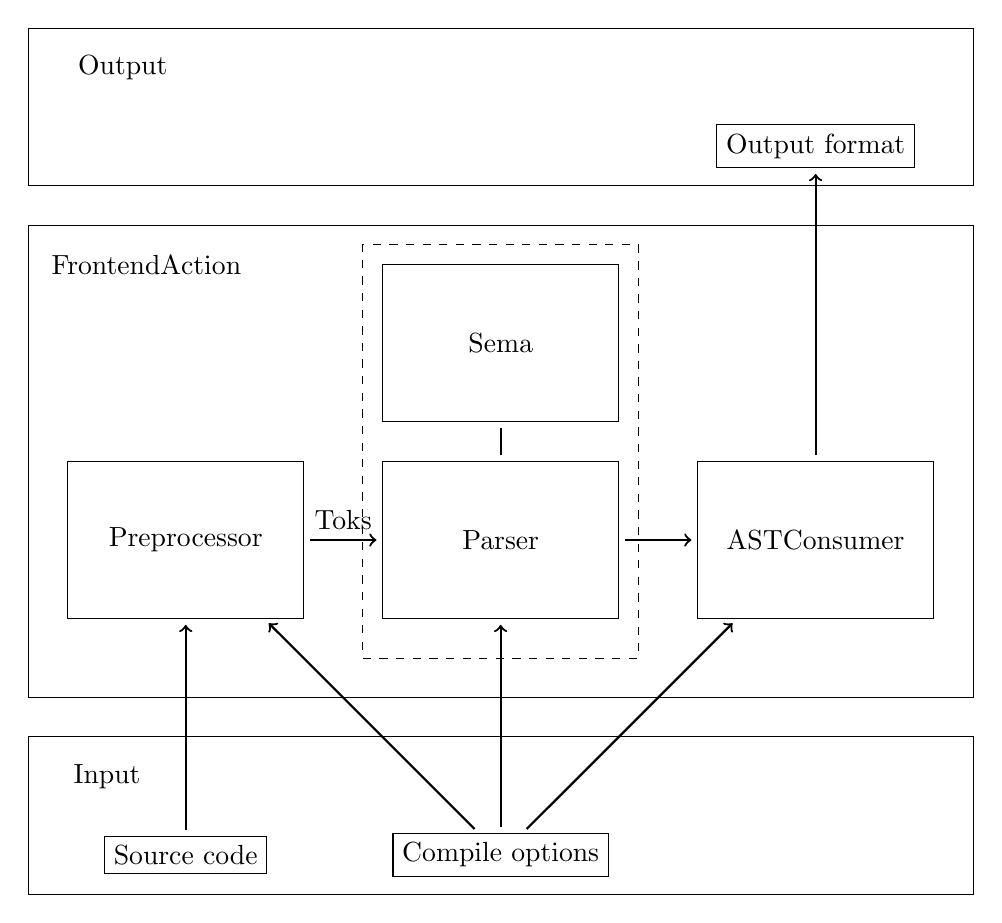
\begin{tikzpicture}
      \node[rectangle] (input) at (1,-1) {Input};
      \node[rectangle,draw] (options) at (6,-2) {Compile options};
      \draw (0,-2.5) -- (12,-2.5) -- (12,-0.5) -- (0,-0.5) -- (0,-2.5);      
      \node[rectangle,draw] (source) at (2,-2) {Source code};

      \node[rectangle] (frontend) at (1.5,5.5) {FrontendAction};
      \draw (0,0) -- (12,0) -- (12,6) -- (0,6) -- (0,0);
      \node[rectangle,draw,minimum height = 2cm, minimum width = 3cm] (lexer)
      at (2,2) {Preprocessor}; 
      \node[rectangle,draw,minimum height = 2cm, minimum width = 3cm]
      (parser) at (6,2) {Parser};
      \node[rectangle,draw,minimum height = 2cm, minimum width = 3cm]
      (sema) at (6,4.5) {Sema}; 
      \node[rectangle,draw,minimum height = 2cm, minimum width = 3cm] (consumer)
      at (10,2) {ASTConsumer};
      \draw[dashed]  (4.25,0.5) -- (7.75,0.5) -- (7.75,5.75) -- (4.25,5.75) --
      (4.25,0.5);
      \draw[thick,shorten <=2pt,shorten >=2pt] (parser) to (sema); 
      
      \draw (0,6.5) -- (12,6.5) -- (12,8.5) -- (0,8.5) -- (0,6.5);
      \node[rectangle,draw] (target) at (10,7) {Output format};
      \node[rectangle] (output) at (1.2,8) {Output};
            
      \draw[->,thick,shorten <=2pt,shorten >=2pt] (lexer) to
      node[pos=0.5,above]{Toks} (parser); 
      \draw[->,thick,shorten <=2pt,shorten >=2pt] (parser) to
      node[pos=0.5,above]{\myast} (consumer);
      \draw[->,thick,shorten <=2pt,shorten >=2pt] (source) to (lexer);
      \draw[->,thick,shorten <=2pt,shorten >=2pt] (options) to (lexer);
      \draw[->,thick,shorten <=2pt,shorten >=2pt] (options) to (parser);
      \draw[->,thick,shorten <=2pt,shorten >=2pt] (options) to (consumer);
      \draw[->,thick,shorten <=2pt,shorten >=2pt] (consumer) to (target);
    \end{tikzpicture}
  \end{center}
  \caption{Clang frontend components}
  \label{fig:clang_frontend}
\end{figure}
The diagram shown in \cref{fig:clang_frontend} illustrates the basic frontend
architecture, which is similar to the architecture shown in
\cref{fig:compiler_frontend}. However, there are notable differences specific to
Clang. 

One significant change is the naming of the lexer. In Clang, the lexer is
referred to as the Preprocessor. This naming convention reflects the fact that
the lexer implementation is encapsulated within the
\mintinline{c++}{Preprocessor} class. This alteration was inspired by the unique
aspects of the C/C++ language, which includes special types of tokens (macros)
that require specialized preprocessing. 

Another noteworthy deviation is found in the parser component. While
conventional compilers typically perform both syntax and semantic analysis
within the parser, Clang distributes these tasks across different
components. The \mintinline{c++}{Parser} component focuses solely on syntax
analysis, while the \mintinline{c++}{Sema} component handles semantic analysis. 

Furthermore, Clang offers the ability to produce output in different forms or
formats. For example, the \mintinline{c++}{CodeGenAction} class serves as the
base class for various code generation actions, such as
\mintinline{c++}{EmitObjAction} or \mintinline{c++}{EmitLLVMAction}. 
%% ./CodeGen/CodeGenAction.h:86:class EmitAssemblyAction : public CodeGenAction {
%% ./CodeGen/CodeGenAction.h:92:class EmitBCAction : public CodeGenAction {
%% ./CodeGen/CodeGenAction.h:98:class EmitLLVMAction : public CodeGenAction {
%% ./CodeGen/CodeGenAction.h:104:class EmitLLVMOnlyAction : public CodeGenAction {
%% ./CodeGen/CodeGenAction.h:110:class EmitCodeGenOnlyAction : public CodeGenAction {
%% ./CodeGen/CodeGenAction.h:116:class EmitObjAction : public CodeGenAction {

We will use the code for \myshell{max} function from \cref{fig:arch_max} for our future exploration of the Clang frontend's internals:
\inputminted{c++}{./src/part1/ch2_arch/max.cpp}
By utilizing the \myshell{-cc1} option, we can directly invoke the Clang frontend,
bypassing the driver. This approach allows us to examine and analyze the inner
workings of the Clang frontend in greater detail. 

\subsection{Preprocessor}

The first part is the \lexer that is called as Preprocessor in Clang.  Its
primary goal is to convert the input program into a stream of tokens. You can
print the token stream using the \myshell{-dump-tokens} options as follows 
\begin{adjustwidth}{0em}{0em}
\begin{verbatim}
$ clang -cc1 -dump-tokens max.cpp
\end{verbatim}
\end{adjustwidth}

The output of the command is as shown below:
% clang -cc1 -dump-tokens ./src/part1/ch2_arch/max.cpp
\begin{adjustwidth}{0em}{0em}
\begin{verbatim}
int 'int'        [StartOfLine]  Loc=<max.cpp:1:1>
identifier 'max'         [LeadingSpace] Loc=<max.cpp:1:5>
l_paren '('             Loc=<max.cpp:1:8>
int 'int'               Loc=<max.cpp:1:9>
identifier 'a'   [LeadingSpace] Loc=<max.cpp:1:13>
comma ','               Loc=<max.cpp:1:14>
int 'int'        [LeadingSpace] Loc=<max.cpp:1:16>
identifier 'b'   [LeadingSpace] Loc=<max.cpp:1:20>
r_paren ')'             Loc=<max.cpp:1:21>
l_brace '{'      [LeadingSpace] Loc=<max.cpp:1:23>
if 'if'  [StartOfLine] [LeadingSpace]   Loc=<max.cpp:2:3>
l_paren '('      [LeadingSpace] Loc=<max.cpp:2:6>
identifier 'a'          Loc=<max.cpp:2:7>
greater '>'      [LeadingSpace] Loc=<max.cpp:2:9>
identifier 'b'   [LeadingSpace] Loc=<max.cpp:2:11>
r_paren ')'             Loc=<max.cpp:2:12>
return 'return'  [StartOfLine] [LeadingSpace]   Loc=<max.cpp:3:5>
identifier 'a'   [LeadingSpace] Loc=<max.cpp:3:12>
semi ';'                Loc=<max.cpp:3:13>
return 'return'  [StartOfLine] [LeadingSpace]   Loc=<max.cpp:4:3>
identifier 'b'   [LeadingSpace] Loc=<max.cpp:4:10>
semi ';'                Loc=<max.cpp:4:11>
r_brace '}'      [StartOfLine]  Loc=<max.cpp:5:1>
eof ''          Loc=<max.cpp:5:2>
\end{verbatim}
\end{adjustwidth}
As we can see, there are different types of tokens, such as language keywords
(e.g., \mintinline{c++}{int}, \mintinline{c++}{return}), identifiers (e.g.,
\mintinline{c++}{max}, \mintinline{c++}{a}, \mintinline{c++}{b}, etc.), and
special symbols (e.g., semicolon, comma, etc.). The tokens for our small program
are called \textbf{normal tokens}, which are returned by the lexer. 

In addition to normal tokens, \clang has an additional type of token called
\textbf{annotation tokens}. The primary difference is that these tokens also
store additional semantic information. For instance, a sequence of normal tokens
can be replaced by the parser with a single annotation token that contains
information about the type or C++ scope. The primary reason for using such
tokens is performance, as it allows for the prevention of reparsing when the
parser needs to backtrack. 

\begin{figure}
  \begin{center}
    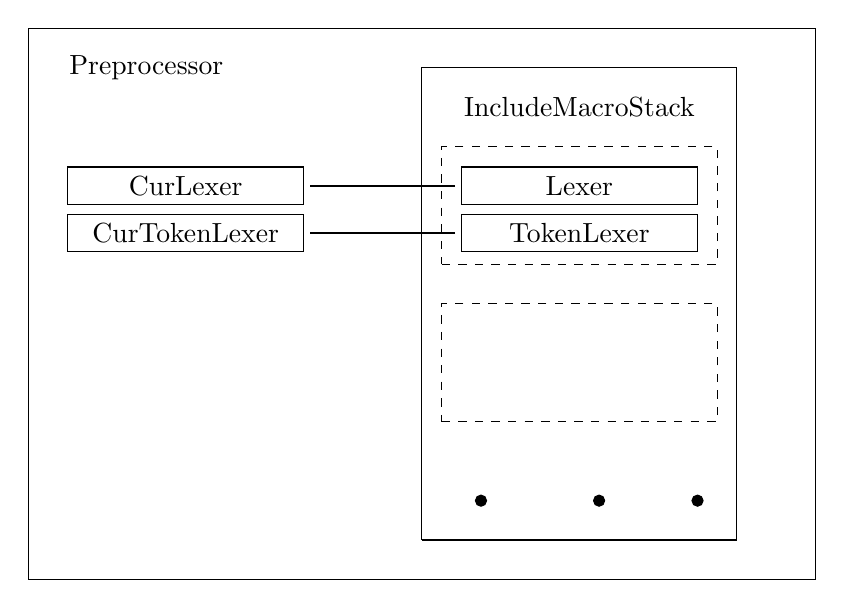
\begin{tikzpicture}
      \node[rectangle] (pp) at (1.5,6.5) {Preprocessor};
      \draw (0,0) -- (10,0) -- (10,7) -- (0,7) -- (0,0);
      \node[rectangle,draw,minimum width = 3cm] (curlexer) at (2,5) {CurLexer};
      \node[rectangle,draw,minimum width = 3cm] (curtokenlexer) at (2,4.4)
           {CurTokenLexer};   

      \node[rectangle] (stack) at (7,6) {IncludeMacroStack};

      \draw (5,0.5) -- (9,0.5) -- (9,6.5) -- (5,6.5) -- (5,0.5);
      \node[rectangle,draw,minimum width = 3cm] (lexer) at (7,5) {Lexer};
      \node[rectangle,draw,minimum width = 3cm] (tokenlexer) at (7,4.4)
           {TokenLexer};
      \draw[dashed]  (5.25,4) -- (8.75,4) -- (8.75,5.5) -- (5.25,5.5) --
      (5.25,4);

      \draw[thick,shorten <=2pt,shorten >=2pt] (lexer) to (curlexer);
      \draw[thick,shorten <=2pt,shorten >=2pt] (tokenlexer) to (curtokenlexer); 
           
      \draw[dashed]  (5.25,2) -- (8.75,2) -- (8.75,3.5) -- (5.25,3.5) --
      (5.25,2);

      \filldraw (5.75,1) circle (2pt);
      \filldraw (8.5,1) circle (2pt);
      \filldraw (7.25,1) circle (2pt);
      
    \end{tikzpicture}
  \end{center}
  \caption{Preprocessor (clang lexer) class internals}
  \label{fig:preprocessor_class}
\end{figure}

C/C++ language has some specifics that influence the internal implementation of
the \mintinline{c++}{Preprocessor} class. The first one is about
macros. The \mintinline{c++}{Preprocessor} class has two different helper
classes to retrieve tokens: 

\begin{itemize}
\item The \mintinline{c++}{Lexer} class is used to convert a text buffer into a
  stream of tokens. 
\item The \mintinline{c++}{TokenLexer} class is used to retrieve tokens from
  macro expansions. 
\end{itemize}

It should be noted that only one of these helpers can be active at a time.

Another specific aspect of C/C++ is the \mintinline{c++}{#include}
directive\footnote{which is also applicable to the import directive}. In this
case, we need to maintain a stack of includes, where each include can have its
own \mintinline{c++}{TokenLexer} or \mintinline{c++}{Lexer}, depending on
whether there is a macro expansion within it. As a result, the
\mintinline{c++}{Preprocessor} class keeps a stack of lexers
(\mintinline{c++}{IncludeMacroStack} class) for each \mintinline{c++}{#include}
directive, as shown in \cref{fig:preprocessor_class}. 

\subsection{Parser and Sema}
The Parser and Sema are crucial components of the \clang compiler frontend. They
handle the syntax and semantic analysis of the source code, producing an \myast
as output. This tree can be visualized for our test program using the command: 

\begin{adjustwidth}{0em}{0em}
\begin{verbatim}
$ clang -cc1 -ast-dump max.cpp
\end{verbatim}
\end{adjustwidth}

The output of this command is shown below
% clang -cc1 -ast-dump ./src/part1/ch2_arch/max.cpp
\begin{adjustwidth}{0em}{0em}
\begin{verbatim}
TranslationUnitDecl 0xc4b578 <<invalid sloc>> <invalid sloc>
|-TypedefDecl 0xc4bde0 <<invalid sloc>> <invalid sloc> implicit __int128_t '__int128'
| `-BuiltinType 0xc4bb40 '__int128'
...
`-FunctionDecl 0xc91580 <max.cpp:1:1, line:5:1> line:1:5 max 'int (int, int)'
  |-ParmVarDecl 0xc91428 <col:9, col:13> col:13 used a 'int'
  |-ParmVarDecl 0xc914a8 <col:16, col:20> col:20 used b 'int'
  `-CompoundStmt 0xc917b8 <col:23, line:5:1>
    |-IfStmt 0xc91750 <line:2:3, line:3:12>
    | |-BinaryOperator 0xc916e8 <line:2:7, col:11> 'bool' '>'
    | | |-ImplicitCastExpr 0xc916b8 <col:7> 'int' <LValueToRValue>
    | | | `-DeclRefExpr 0xc91678 <col:7> 'int' lvalue ParmVar 0xc91428 'a' 'int'
    | | `-ImplicitCastExpr 0xc916d0 <col:11> 'int' <LValueToRValue>
    | |   `-DeclRefExpr 0xc91698 <col:11> 'int' lvalue ParmVar 0xc914a8 'b' 'int'
    | `-ReturnStmt 0xc91740 <line:3:5, col:12>
    |   `-ImplicitCastExpr 0xc91728 <col:12> 'int' <LValueToRValue>
    |     `-DeclRefExpr 0xc91708 <col:12> 'int' lvalue ParmVar 0xc91428 'a' 'int'
    `-ReturnStmt 0xc917a8 <line:4:3, col:10>
      `-ImplicitCastExpr 0xc91790 <col:10> 'int' <LValueToRValue>
        `-DeclRefExpr 0xc91770 <col:10> 'int' lvalue ParmVar 0xc914a8 'b' 'int'
\end{verbatim}
\end{adjustwidth}

Clang utilizes a hand-written recursive-descent parser
\citep{llvm:clangfeatures}. This parser can be considered simple, and this
simplicity was one key reason for its selection. Additionally, the complex rules
specified for the C/C++ languages necessitated an ad-hoc parser with easily
adaptable rules. 

Let's explore how this works with our example. Parsing begins with a top-level
declaration known as a \mintinline{c++}{TranslationUnitDecl}, representing a
single translation unit. The C++ standard defines a translation unit as follows
\citep[lex.separate]{standard:cpp20}: 

\begin{quote}
A source file together with all the headers (16.5.1.2) and source files included
(15.3) via the preprocessing directive \#include, less any source lines skipped
by any of the conditional inclusion (15.2) preprocessing directives, is called a
translation unit. 
\end{quote}

The parser first recognizes that the initial tokens from the source code
correspond to a function definition, as defined in the C++ standard
\citep[dcl.fct.def.general]{standard:cpp20}: 

% https://eel.is/c++draft/dcl.fct.def.general#nt:function-definition
\begin{adjustwidth}{0em}{0em}
\begin{verbatim}
function-definition :
        ... declarator ... function-body
        ...
\end{verbatim}
\end{adjustwidth}
The corresponding code is below
\begin{minted}{c++}
int max(...) {
  ...
}
\end{minted}
The function definition necessitates a declarator and function body. We'll start
with the declarator, defined in the C++ standard as
\citep[dcl.decl.general]{standard:cpp20}: 

% https://eel.is/c++draft/dcl.decl.general#nt:declarator
\begin{adjustwidth}{0em}{0em}
\begin{verbatim}
declarator:
        ...
        ... parameters-and-qualifiers ...
...
parameters-and-qualifiers:
        ( parameter-declaration-clause ) ...
...
parameter-declaration-clause:
        parameter-declaration-list ...
parameter-declaration-list:
        parameter-declaration
        parameter-declaration-list , parameter-declaration
\end{verbatim}
\end{adjustwidth}
In other words, the declarator specifies a list of parameter declarations within
brackets. The corresponding piece of code from the source is as follows: 
\begin{minted}{c++}
... (int a, int b) 
  ...
\end{minted}

The function definition, as stated above, also requires a function body. The C++
standard specifies the function body as follows: 
% https://eel.is/c++draft/dcl.fct.def.general#nt:function-body
\citep[dcl.fct.def.general]{standard:cpp20}
\begin{adjustwidth}{0em}{0em}
\begin{verbatim}
function-body:
       ... compound-statement
       ...
\end{verbatim}
\end{adjustwidth}
Thus the function body consists of a compound statement, which is defined as follows in the C++ standard \citep[stmt.block]{standard:cpp20}
% https://eel.is/c++draft/stmt.block#nt:compound-statement
\begin{adjustwidth}{0em}{0em}
\begin{verbatim}
compound-statement:
       { statement-seq ... }
statement-seq:
       statement
       statement-seq statement
\end{verbatim}
\end{adjustwidth}
Therefore, it describes a sequence of statements enclosed within
\mintinline{c++}{{...}} brackets. 

Our program has two types of statements: the conditional (if) statement and the
return statement. These are represented in the C++ grammar definition as follows
\citep[stmt.pre]{standard:cpp20}: 
% https://eel.is/c++draft/stmt.pre#nt:statement
\begin{adjustwidth}{0em}{0em}
\begin{verbatim}
statement:
        ...
        selection-statement
        ...
        jump-statement
        ...
\end{verbatim}
\end{adjustwidth}
In this context, the selection statement corresponds to the \mintinline{c++}{if}
condition in our program, while the jump statement corresponds to the
\mintinline{c++}{return} operator. 

Let's examine the jump statement in more detail
\citep[stmt.jump.general]{standard:cpp20}: 
% https://eel.is/c++draft/stmt.jump.general#nt:jump-statement
\begin{adjustwidth}{0em}{0em}
\begin{verbatim}
jump-statement:
        ...
        return expr-or-braced-init-list;
        ...
\end{verbatim}
\end{adjustwidth}
where expr-or-braced-init-list is defined as
\citep[dcl.init.general]{standard:cpp20}: 
% https://eel.is/c++draft/dcl.init.general#nt:expr-or-braced-init-list
\begin{adjustwidth}{0em}{0em}
\begin{verbatim}
expr-or-braced-init-list:
        expression
        ...
\end{verbatim}
\end{adjustwidth}
In this context, the \mintinline{c++}{return} keyword is followed by an
expression and a semicolon. In our case, there's an implicit cast expression
that automatically converts the variable into the required type (int). 

It can be enlightening to examine the parser's operation through the \lldb
debugger: 
% lldb ./llvm-project-16.x/build/bin/clang -- -cc1 src/part1/ch2_arch/max.cpp
\begin{figure}[H]
\begin{minted}{shell-session}
$ lldb <...>/llvm-project/build/bin/clang -- -cc1 max.cpp
...  
(lldb) b clang::Parser::ParseReturnStatement
(lldb) r
...
(lldb) c
...
* thread #1, name = 'clang', stop reason = breakpoint 1.1
    frame #0: ... clang::Parser::ParseReturnStatement(...) at ParseStmt.cpp:2358:3
   2355 ///         'co_return' expression[opt] ';'
   2356 ///         'co_return' braced-init-list ';'
   2357 StmtResult Parser::ParseReturnStatement() {
-> 2358   assert((Tok.is(tok::kw_return) || Tok.is(tok::kw_co_return)) &&
   2359          "Not a return stmt!");
   2360   bool IsCoreturn = Tok.is(tok::kw_co_return);
   2361   SourceLocation ReturnLoc = ConsumeToken();  // eat the 'return'.
(lldb) bt
  * frame #0: ... clang::Parser::ParseReturnStatement( ...
    ... 
    frame #2: ... clang::Parser::ParseStatementOrDeclaration( ...
    frame #3: ... clang::Parser::ParseCompoundStatementBody( ...
    frame #4: ... clang::Parser::ParseFunctionStatementBody( ...
    frame #5: ... clang::Parser::ParseFunctionDefinition( ...
...
\end{minted}
\caption{Second return statement parsing at max.cpp example program}
\label{fig:lldb_parser}
\end{figure}
As you can see in \cref{fig:lldb_parser}, line 3, we've set a breakpoint for the
parsing of return statements\footnote{Specifically, at the
\mintinline{c++}{clang::Parser::ParseReturnStatement} method}. Our program has
two return statements. We bypass the first call (line 6) and halt at the second
method invocation (line 13). The backtrace (from the 'bt' command at line 17)
displays the call stack for the parsing process. This stack mirrors the parsing
blocks we described earlier, adhering to the C++ grammar detailed in
\citep[lex.separate]{standard:cpp20}. 

The parsing results in the generation of AST. We can
also inspect the process of AST creation using the debugger. To do this, we need
to set a corresponding breakpoint at the
\mintinline{c++}{clang::ReturnStmt::Create} method: 
% lldb ./llvm-project-16.x/build/bin/clang -- -cc1 src/part1/ch2_arch/max.cpp
\begin{minted}{shell-session}
$ lldb <...>/llvm-project/build/bin/clang -- -cc1 max.cpp
...
(lldb) b clang::ReturnStmt::Create
(lldb) r
...
(lldb) c
...  
* thread #1, name = 'clang', stop reason = breakpoint 1.1
    frame #0: ... clang::ReturnStmt::Create(...) at Stmt.cpp:1204:8
   1201 
   1202 ReturnStmt *ReturnStmt::Create( ... ) {
-> 1204   bool HasNRVOCandidate = NRVOCandidate != nullptr;
   1205   ...
   1206   ...
   1207   return new (Mem) ReturnStmt(RL, E, NRVOCandidate);
(lldb) bt
* thread #1, name = 'clang', stop reason = breakpoint 1.1
  * frame #0: ... clang::ReturnStmt::Create( ...
    frame #1: ... clang::Sema::BuildReturnStmt( ...
    frame #2: ... clang::Sema::ActOnReturnStmt( ...
    frame #3: ... clang::Parser::ParseReturnStatement( ...
    frame #4: ... clang::Parser::ParseStatementOrDeclarationAfterAttributes( ...
    ...
\end{minted}
As can be seen, the AST node for the return statement is created by the Sema
component. 

The beginning of the return statement parser can be located in frame 4:
\begin{minted}{shell-session}
(lldb) f 4
frame #4: ... clang::Parser::ParseStatementOrDeclarationAfterAttributes( ...
   325      break;
   326    case tok::kw_return:              // C99 6.8.6.4: return-statement
-> 327      Res = ParseReturnStatement();
   328      SemiError = "return";
   329      break;
   330    case tok::kw_co_return:            // C++ Coroutines: ...
(lldb) 
\end{minted}
As we can observe, there is a reference to the C99 standard \citep{standard:c99}
for the corresponding statement. The standard \citep{standard:c99} provides a
detailed description of the statement and the process for handling it. 

The code assumes that the current token is of type
\mintinline{c++}{tok::kw_return}, and in this case, the parser invokes the
relevant \mintinline{c++}{clang::Parser::ParseReturnStatement} method. 

While the process of AST node creation can vary across different C++ constructs,
it generally follows the pattern displayed in \cref{fig:parse_step}. 
\begin{figure}[H]
    \begin{center}
      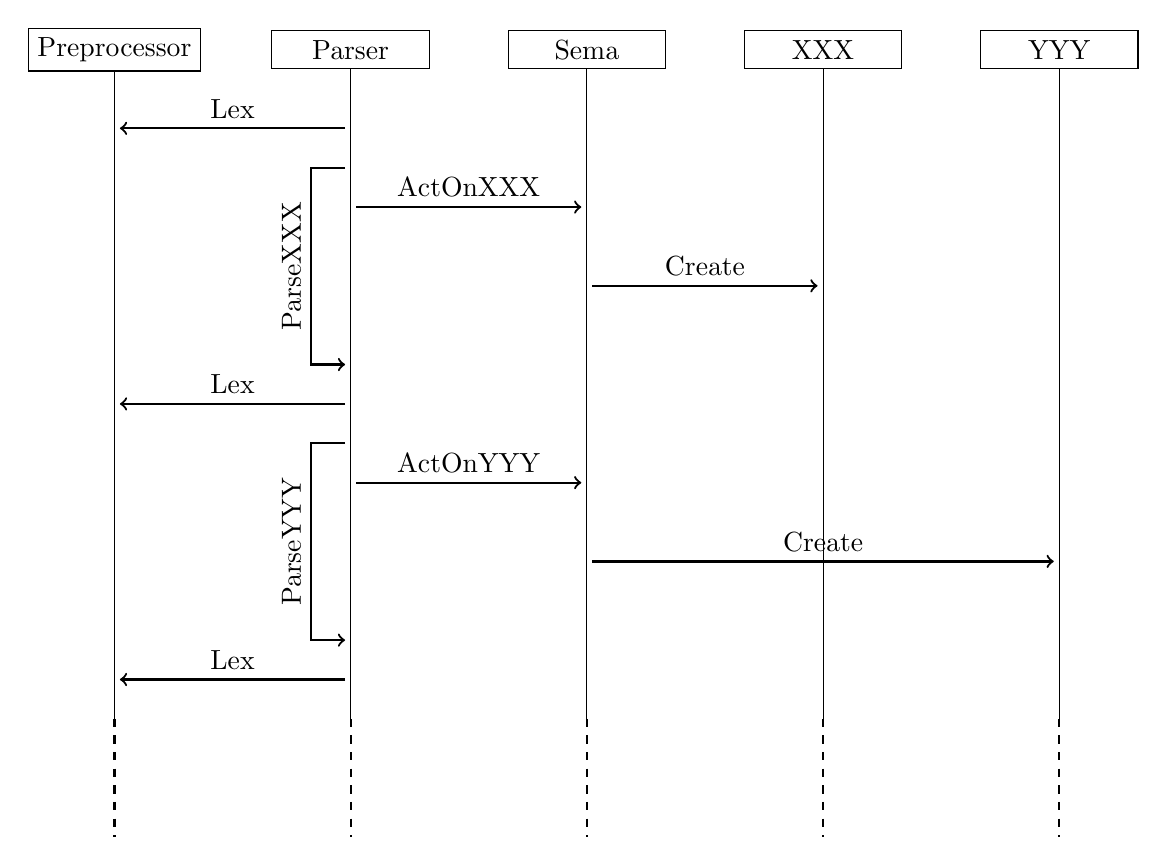
\begin{tikzpicture}
      \node[rectangle,draw,minimum width = 2cm] (preprocessor) at (0,10)
           {Preprocessor};
      \draw (preprocessor) -- (0,1.5);
      \draw[thick,dashed] (0,1.5) to (0,0);
      \node[rectangle,draw,minimum width = 2cm] (parser) at (3,10)
           {Parser};
      \draw (parser) -- (3,1.5);
      \draw[thick,dashed] (3,1.5) to (3,0);
      
      \node[rectangle,draw,minimum width = 2cm] (sema) at (6,10)
           {Sema};
      \draw (sema) -- (6,1.5);
      \draw[thick,dashed] (6,1.5) to (6,0);     
      \node[rectangle,draw,minimum width = 2cm] (xxx) at (9,10)
           {XXX};
      \draw (xxx) -- (9,1.5);
      \draw[thick,dashed] (9,1.5) to (9,0);          
      \node[rectangle,draw,minimum width = 2cm] (yyy) at (12,10)
           {YYY};
      \draw (yyy) -- (12,1.5);
      \draw[thick,dashed] (12,1.5) to (12,0);     

      \draw[->,thick,shorten <=2pt,shorten >=2pt] (3,9) to
      node[pos=0.5,above]{Lex} (0,9);

      \draw[->,thick,shorten <=2pt,shorten >=2pt] (3,8.5) to (2.5,8.5) to
      node[pos=0.5,above, rotate=90]{ParseXXX} (2.5,6) to (3,6);

      \draw[->,thick,shorten <=2pt,shorten >=2pt] (3,8) to
      node[pos=0.5,above]{ActOnXXX} (6,8);

      \draw[->,thick,shorten <=2pt,shorten >=2pt] (6,7) to
      node[pos=0.5,above]{Create} (9,7);

      \draw[->,thick,shorten <=2pt,shorten >=2pt] (3,5.5) to
      node[pos=0.5,above]{Lex} (0,5.5);

      \draw[->,thick,shorten <=2pt,shorten >=2pt] (3,5) to (2.5,5) to
      node[pos=0.5,above, rotate=90]{ParseYYY} (2.5,2.5) to (3,2.5);

      \draw[->,thick,shorten <=2pt,shorten >=2pt] (3,4.5) to
      node[pos=0.5,above]{ActOnYYY} (6,4.5);

      \draw[->,thick,shorten <=2pt,shorten >=2pt] (6,3.5) to
      node[pos=0.5,above]{Create} (12,3.5);

      \draw[->,thick,shorten <=2pt,shorten >=2pt] (3,2) to
      node[pos=0.5,above]{Lex} (0,2);      
    \end{tikzpicture}
  \end{center}
  \caption{C++ parsing in Clang frontend}
  \label{fig:parse_step}
\end{figure}
As can be seen, the \mintinline{c++}{Parser} invokes the
\mintinline{c++}{Preprocessor::Lex} method to retrieve a token from the
lexer. It then calls a method corresponding to the token, for example,
\mintinline{c++}{Parser:ParseXXX} for the token \mintinline{c++}{XXX}. This
method then calls \mintinline{c++}{Sema::ActOnXXX}, which creates the
corresponding object using \mintinline{c++}{XXX::Create}. The process is then
repeated with a new token. 

With this, we have now fully explored how the typical compiler frontend flow is
implemented in Clang. We can see how the lexer component (the preprocessor)
works in tandem with the parser (which comprises the parser and sema components)
to produce the primary data structure for future code generation: the Abstract
Syntax Tree (AST). The AST is not only essential for code generation but also
for code analysis and modification. Clang provides easy access to the AST,
thereby enabling the development of a diverse range of compiler tools. 

\section{Summary}

In this chapter, we have acquired a basic understanding of compiler architecture
and delved into the various stages of the compilation process, with a focus on
the Clang driver. We have explored the internals of the Clang frontend, studying
the preprocessor that transforms a program into a set of tokens, and the parser,
which interacts with a component called 'Sema'. Together, these elements perform
syntax and semantic analysis. 

The upcoming chapter will center on the Clang Abstract Syntax Tree (AST)—the
primary data structure employed in various Clang tools. We will discuss its
construction and the methods for traversing it. 

\section{Further reading}
\begin{itemize}
\item Working Draft, Standard for Programming Language C++:
  https://eel.is/c++draft/ 
\item ``Clang'' CFE Internals Manual:
  https://clang.llvm.org/docs/InternalsManual.html
\item Keith Cooper and Linda Torczon: Engineering A Compiler, 2012
  \citep{book:engineering_a_compiler} 
\end{itemize}
